 \documentclass{article}
\usepackage{graphicx}
\usepackage[german]{babel}
\usepackage{amsmath,amssymb,amscd}
\usepackage{float}
\usepackage{makeidx}
\usepackage{etoolbox}
\usepackage{pythonhighlight}

\oddsidemargin 0.0in 
\evensidemargin 1.0in 
\textwidth 6.0in 
\headheight 0.0in 
\topmargin 0.0in 
\textheight 9.0in 

\begin{document}
\section*{Mathematik f\"ur Informatiker - \"Ubungsblatt 0}
\subsection*{Python, Jupyter Notebooks und Grundlagen der Programmierung}
Die Vorlesung \textit{Mathematik f\"ur Informatiker} folgt in weiten Teilen dem Buch \textit{Konkrete Mathematik (nicht nur) f\"ur Informatiker} von Edmund Weitz \cite{weitz}. Dieses Buch verfolgt den Ansatz, dass Informatiker*innen in ihrem sp"ateren Berufsleben mehr angewandte (konkrete) Mathematik ben"otigen wie \glqq reine\grqq{} Mathematik, welche Mathematik der Mathematik wegen betreibt. Anwendungswerkzeug der Wahl: Programmieren! Sie lernen in meiner Vorlesung die mathematischen Begriffe, Methoden und vor allem deren Anwendungen, indem sie diese in Computerprogramme \glqq "ubersetzen\grqq. Wir werden daf"ur (wie auch Herr Weitz) Python und Jupyter Notebooks verwenden. 
\\\\
\textbf{Python} is an easy to learn, powerful programming language. It has efficient high-level data structures and a simple but effective approach to object-oriented programming. \cite{pythonwebsite}
\\\\
The \textbf{Jupyter Notebook} is an open-source web application that allows you to create and share documents that contain live code, equations, visualizations and narrative text. \cite{jupyterwebsite}
\\\\
Die Installation von Python und Jupyter ist recht einfach - vorausgesetzt sie verwenden daf"ur wie von Herr Weitz vorgeschlagen Docker: 
\\

http://weitz.de/install/
\\\\
Falls sie lieber Python direkt auf ihrem Betriebssystem laufen lassen m"ochten ist dies nat"urlich auch m"oglich... am einfachsten unter Linux ;-)... ist ihr Grundbetriebssystem Windows (so wie bei mir), k"onnen sie entweder mit einer virtuellen Maschine (z.B. VMWare) oder mit dem Windows Subsystem for Linux (WSL) arbeiten. "Offnen sie dann auf Linux ein Terminal und installieren sie Miniconda wir hier beschrieben: 
\\

https://docs.conda.io/projects/conda/en/latest/user-guide/install/linux.html\\\\
Nun sollten sie (nach Neustart des Terminals) mit 
\begin{verbatim}
  conda install jupyterlab
\end{verbatim}
jupyterlab installieren und danach mit 
\begin{verbatim}
  jupyter notebook
\end{verbatim}
ihr erstes Jupyter-Notebook erstellen (new-Button) und ihr erstes Python-Programm (nat"urlich die Ausgabe von Hello World!) damit schreiben k"onnen:
\begin{figure}[H]
\centering
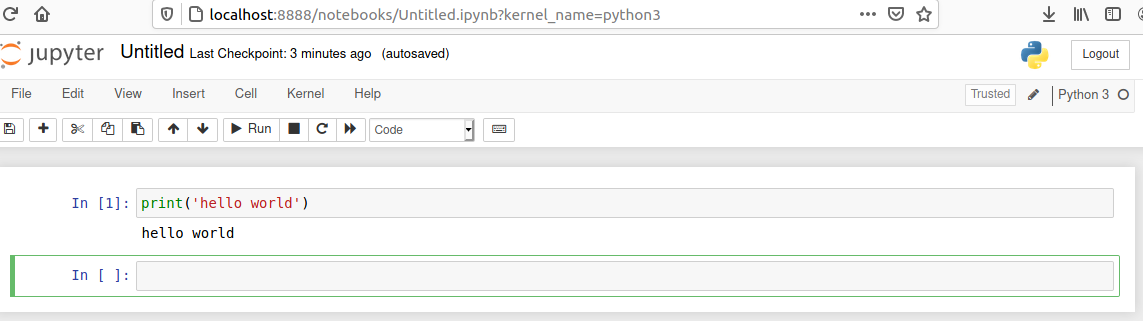
\includegraphics[width=0.9\columnwidth]{jupyternotebookhelloworld.png}
\end{figure}\noindent
Wenn sie was "ahnliches wie im obigen Bild auf ihrem Bildschirm sehen, haben sie den ersten Schritt zum Erlernen der linearen Algebra und der Grundlegenden der Analysis mittels Programmieren geschafft $\rightarrow$ Herzlichen Gl"uckwunsch!
\\\\
Vielleicht fragen sie sich, warum ich hier nicht nur einen Weg f"ur die Installation von Jupyter angegeben habe, der dann f"ur alle funktioniert. 
Nun, das liegt zum Einen daran, dass ich ihr \glqq Setup\grqq{} (Rechner, Betriebssystem, ...) nicht kenne, zum Anderen darin, dass sie sich zu Informatiker*innen 
ausbilden lassen und sich m"oglichst fr"uh daran gew"ohnen sollten, dass es meist nicht \glqq den einen richtigen Weg\grqq{}
zur L"osung einer Aufgabenstellung gibt, sondern mehrere Wege, welche alle zu einem akzeptablen Ergebnis f"uhren. Dies gilt nicht nur f"ur die 
Auswahl von Werkzeugen (so wie hier), sondern insbesondere auch bei der Architektur von Software bzw. deren Implementierung.
\\\\
Nun ben"otigen wir noch einige programatische Grundlagen in Python die sie schon aus anderen Vorlesungen kennen sollten. Falls nicht, auch nicht schlimm! Dann haben sie die Chance sie hier zu lernen.

\subsection*{Funktionen und Schleifen}
Lassen sie uns zuerst eine Funktion schreiben, welche die Summe der ersten $n$ nat"urlichen Zahlen berechnet. Passen sie dazu folgenden Python-Code so an (ersetzen sie \verb+...+ durch den richtigen Befehl), dass der Aufruf \verb+sumFn(5)+ das richtige Ergebnis ($1+2+3+4+5 = 15$) liefert:

\begin{python}
def sumFn(n):
    i = 0
    s = 0
    while i <= n:
        ...
        i = i +1
    return s
sumFn(5)

\end{python}
Erweitern sie die Funktion nun so, dass sie alle Zwischenresultate ausgibt:
\begin{figure}[H]
\centering
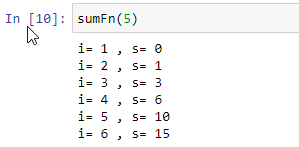
\includegraphics{sumFnOutput.png}
\end{figure} \noindent
Sie sollte nun wissen,
\begin{itemize}
\item wie sie in Python Funktionen definieren und diese aufrufen k"onnen,
\item wie die while-Schleife funktioniert und
\item wie sie in Python Text und Variableninhalte gemeinsam ausgeben k"onnen.
\end{itemize}
Erweitern sie die Funktion \verb+sumFn(n)+ nun so, dass sie auch f"ur negative Werte etwas \glqq sinnvolles\grqq{} zur"uckgibt (also z.B. f"ur \verb+-4+ den Wert \verb+-10+). Hinweis: sie k"onnen Funktionen auch aus Funkionen aufrufen!


\subsection*{Anonyme(Lambda) Funktionen}
Bisher haben wir unseren Funkionen immer Namen gegeben. In Python kann man aber auch ''Namenlose'' (== Anonyme) Funktionen
mit Hilfe des reservierten Worts {\verb+lambda+} definieren. Dies ist besonders dann hilfreich, wenn man einer Funktion eine
anderen Funktion als Parameter "ubergeben m"ochte, z.B. um diese gleich f"ur mehrere Werte auswerten zu lassen.

So k"onnen wir zum Beispiel eine Funktion schreiben, die eine anonyme Funktion $f$, die ihr als Parameter "ubergeben wird, f"ur
alle ganzzahligen Werte zwischen $a$ und $b$ (die wir ebenfalls als Parameter "ubergeben) auswertet:

\begin{python}
def evaluate (f, a, b):
  return [f(x) for x in range(a, b)]
\end{python}

Rufen wir nun die Funktion {\verb+evaluate+} mit den Parameter {\verb+lambda x: x * x+}, $2$ und $5$ auf. Sie sollten
als Ausgabe {\verb+[4, 9, 16]+} bekommen.

Spielen sie ein wenig mit der Funktion {\verb+evaluate+} herum indem sie unterschiedliche Funktionen (z.B. $\frac{1}{x}$ oder auch $e^x$) 
und Wertebereiche "ubergeben. 
\\Hinweis: Implementieren sie die Exponential-Funktion (noch :-)) nicht selbst sondern verwenden sie die Mathematik-Bibliothek (\verb+import math+) von Python.

Schreiben sie die Funktion derart um, dass auch der Parameter $b$ mit in die Auswertung aufgenommen wird.

Sie k"onnen in Python auch Funktion als Paremeter "ubergeben. So k"onnen wir obiges Ergebnis auch mit
\begin{python}
def sqrt(x):
    return x * x
evaluate (sqrt, 2, 5)
\end{python}
berechnen. 

\subsection*{Funktionen Zeichnen}
Oft hilft es enorm eine mathematische Funktion zu \glqq Zeichnen\grqq{} um sie besser zu \glqq verstehen\grqq{}. Herr Weitz hat zum Plotten von mathematischen Funktionen eine eigene Biblithek (\verb+plot+) geschrieben, welche einen \textit{wrapper} f"ur die etwas schwieriger anzuwendende Bibliothek \verb+mathplotlib+ bildet. Wenn sie \verb+Jupyter+ im Docker von Herr Weitz laufen lassen, ist diese Bibliothek bereits \glqq installiert \grqq{}. Falls nicht, finden sie seine Bibliothek auf seiner Homepage. Ist alles richtig installiert, sollten sie mit 
\begin{python}
from plot import *
plotFunc2D(lambda x: x*x + x - 1, [-2.5, 1.5])
\end{python}
einen Plot der Funktion $f(x) = x^2 + x -1$ in karthesischen Koordinaten erhalten:
\begin{figure}[H]
\centering
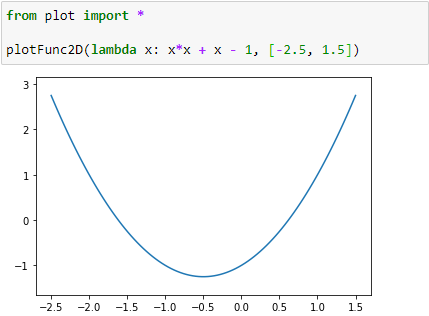
\includegraphics[width=0.9\columnwidth]{sqrtxplot.png}
\end{figure}\noindent
Solche Plots werden Funktionsgraphen oder nur Graphen genannt. Versuchen sie mit den Parametern \verb+grid=True+ und \verb+scaled=True+ den Plot zu beeinflussen. Plotten sie auch andere ihnen 
bekannte Funktionen um sich an den Umgang mit \verb+plotFunc2D+ zu gew"ohnen.

Nun gibt es aber Kurven in der Ebene, die sich \textit{nicht} als Graph einer Funktionen darstellen lassen, da sie einem Punkt der $x$-Achse merhrere Punkte in der $x$-$y$-Ebene zuweisen. Dies gilt z.B. f"ur den Einheitskreis $x^2 + y^2 = 1$. Falls sie versuchen diese Funktion umzuformen und mit \verb+plotFunc2D(lambda x: math.sqrt(x*x - 1), [-2.5, 1.5])+) zu plotten, k"onnen sie zwar einiges "uber die Internas der Plot-Bibliothek erfahren, werden aber keinen Graph des Einheitskreises erhalten. Hier schafft die Parameterdarstellung Abhilfe, in der man die Punkte des Einheitskreises als Vektor abh"angig von einem Parameter $t$ (dem Winkel) darstellt
$$
  \vec{r}(t) = \begin{pmatrix} x(t) \\ y(t)\end{pmatrix} = \begin{pmatrix} \cos(t) \\ \sin(t)\end{pmatrix}.
$$
Machen sie sich keine Sorgen wenn sie das (noch) nicht ganz verstehen! Wir werden die Parameterdarstellung noch ausf"uhrlich behandeln. In dieser Darstellung k"onnen wir den Einheitskreis nun unter Verwendung der Funktion \verb+plotCurve2D+ Plotten, indem wir f"ur jeden Parameter $t$ zwei Werte (einen f"ur $x(t)$ und einen f"ur $y(t)$) angeben:
\begin{python}
plotCurve2D(lambda t: (math.cos(t), math.sin(t)), [0, 2*math.pi])
\end{python}
Versuchen sie nun, einen Kreis mit Mittelpunkt $(1,1)$ und Radius $\pi$ zu zeichnen.

Die Bibliothek \verb+plot+ kann noch viel mehr, unter anderem 3D-Plots, H"ohenlinien oder auch Konturdiagramme zeichnen. So wir diese Plots brauchen werden wir sie einf"uhren. Wenn sie in ihrem Setup eine einfache mathematische Funktoin plotten k"onnen, reicht das zum jetzigen Zeitpunkt vollkommen.
\subsection*{Listen und Generatoren}
In Python kann man Listen sehr einfach erzeugen. So weist die Eingabe 
\begin{python}
a = [1,2,3], b = ['a', 'b', 'c']
\end{python}
der Variable {\verb+a+} eine Liste mit den drei Integer-Werten \verb+1+, \verb+2+ und \verb+3+ zu, 
die Variable {\verb+b+} bekommt eine Liste mit den drei Buchstaben \verb+a+, \verb+b+ und \verb+c+ zugewiesen.
"Uber Listen kann man nun \textit{iterieren} (== die Elemente der Liste einzeln durchgehen):
\begin{python}
for i in a:
  print(i)
1
2
3
\end{python}
oder auch unterschiedliche Operatoren anwenden:
\begin{python}
a.append(5), a.revert(), reversed(a), a.insert(3, 4), count(a), ... 
\end{python}
Spielen sie ein wenig mit den Operatoren (auch mit den hier nicht angef"uhrten, aber auf der Python-Seite \cite{pythonwebsite} angegebenen) herum und machen sie sich den Umgang mit Listen zu eigen.
Wir werden sie in der linearen Algebra intensiv f"ur die Darstellung von Vektoren und Matrizen
verwenden.

Mit dem Schl"usselwort \verb+in+ k"onnen sie pr"ufen, ob ein Element in der Liste vorhanden ist. Der Aufruf
\begin{python}
10 in a, 1 in a
\end{python}
sollte \verb+(False, True)+ liefern.

Neben der Angabe von einzelnen Elementen k"onnen wir Listen auch mit dem Befehl Range erzeugen.
F"ur die Eingabe von
\begin{python}
a = list(range(5))
b = list(range(2,6))
c = list(range(2,10,2))
\end{python}
bekommen wir \verb+[0, 1, 2, 3, 4]+, \verb+[2, 3, 4, 5]+ und \verb+[2, 4, 6, 8]+. Bitte studieren sie
auch hier die Python-Dokumentation \cite{pythonwebsite} falls sie sich nicht sicher sind was die einzelnen Parameter zu bedeuten haben. Python kann auch "uber Objekte vom Typ Range iterieren $\rightarrow$ lassen sie bitte das \verb+list+ weg, wenn sie "uber einen mit Range erzeugen Bereich iterieren m"ochten (sie werden am Ende dieses Abschnitts verstehen warum dies besser ist).
\\\\
Von der Syntax her besonders \textit{elegent} finde ich den Zugriff auf Listenelementen in Python. F"ur
\begin{python}
a = list(range(5))
a[1:3], a[3:5], a[-2], a[3:-1], a[0], a[-1]
\end{python}
sollten sie \verb+([1, 2], [3, 4], 3, [3], 0, 4)+  als Ausgabe bekommen. Auch hier empfielt sich das Studium der Python-Dokumentation \cite{pythonwebsite} falls ihnen z.B. der negative Index nicht ganz geheuer ist.
\\\\
Lassen sie uns zu guter letzt noch ein weiteres (meiner Meinung nach sehr \textit{sch"ones}, aber zumindest sehr n"utzliches) Sprachkonstrukt von Python - \textbf{Generatoren} - anschauen. "Uberlegen sie sich dazu in einem ersten Schritt, was folgende Funktion 
\begin{python}
def first_n(n):
   num, nums = 0, []
   while num < n:
       nums.append(num)
       num += 1
   return nums
\end{python}
bei dem Aufruf \verb+sum(first_n(1000000))+ mit dem Hauptspeicher ihres Rechners \glqq anstellt\grqq{}. Wenn sie zu dem Schluss \glqq nichts gutes!\grqq{} kommen, liegen sie richtig. Der Aufruf dieser Methode \glqq zwingt\grqq{} Python dazu, alle $1000000$ Werte im Hauptspeicher abzulegen und als Resultat zur"uckzuliefern $\rightarrow$ sehr ineffizient! Da einer der Hauptanwendungen von Listen darin besteht, auf den einzelnen Listenelementen \glqq der Reihe nach\grqq{} Operationen auszuf"uhren (== durch die Liste zu iterieren), ist es im Allgemeinen (so auch in unserer speziellen Anwendung, dem Bilden der Summe "uber alle Werte) nicht notwendig, alle Elemente auf einmal zur"uckzuliefern. Wir k"onnen die Elemente zu dem Zeitpunkt \textit{generieren} zu dem wir sie ben"otigen $\rightarrow$ genau dies machen in Python Generatoren f"ur uns:
\begin{python}
def firstn(n):
    num = 0
    while num < n:
        yield num
        num += 1
\end{python}
Diese Funktion liefert nun keine Liste mehr zur"uck, sondern aufgrund des \verb+yield+-Ausdrucks einen Generator "uber den wir iterieren k"onnen. Das Resultat von \verb+sum(firstn(1000000))+ sollte mit dem obigen Aufruf "Ubereinstimmen ($499999500000$), nur die Berechnung ist auf diese Art wesentlich effizienten!
Neben dem geringeren Speicherverbrauch f"uhrt das Verwenden von \verb+yield+ auch zu einem verbesserten Laufzeitverhalten (== wir ben"otigen weniger Zeit zum Berechnen der Summe). Die ben"otigte Zeit zum Ausf"uhren von Python-Code kann man sehr einfach mit der Funktion \verb+timeit+ ermitteln:
\begin{python}
import timeit

n = 1000000

starttime = timeit.default_timer()
sum(first_n(n))
print('Execution time of "sum(first_n(n))":', timeit.default_timer() - starttime)
starttime = timeit.default_timer()
sum(firstn(n))
print('Execution time of "sum(firstn(n))":', timeit.default_timer() - starttime)
\end{python}
F"uhren sie diesen Code \glqq ein paar mal\grqq{} aus $\rightarrow$ sie sollten feststellen k"onnen, dass die Funktion \verb+firstn(n)+ im Mittel nur halb soviel Zeit ben"otigt wie die Funktion \verb+first_n(n)+.

Wenn ich ihnen nun noch sage, dass der Befehl \verb+Range(5)+ keine Liste sondern einen Generator liefert, sollte mein \glqq Versprechen\grqq{} von etwas weiter oben eingel"ost sein und sie verstehen, warum es besser ist, "uber \verb+range(5)+ zu iterieren wie "uber \verb+list(range(5))+.

Wenn sie bis hierher folgen konnten und die Beispiele selbst"andig ausgef"uhrt und auch ein wenig mit Python experimentiert haben, sollten sie in der Lage sein, folgenden Code zu verstehen:
\begin{python}
def someValues(seq, L = [10 ** k for k in range(10)]):
    for n in L:
        print("{:>15}: {}".format(n, seq(n)))
        
someValues(lambda n: n / (n + 1))
\end{python}
Wir werden diese Funktion sp"ater in der Analysis be"otigen um auf einfache Art pr"ufen zu k"onnen, wie sich eine mathematische Funktion (im Beispiel $\frac{n}{n +1}$) \glqq verh"alt\grqq{}. Zum jetzigen Zeitpunkt ist aber nur wichtig, dass sie die eingef"uhrten Python-Konstrukte gut genug verinnerlicht haben, um die Funktionsweise von \verb+someValues+ verstehen zu k"onnen. Ist dies der Fall, k"onnen sie sich in der Vorlesung und den Seminaren voll auf die Mathematik konzentrieren und dem Erlernen der Linearen Algebra sowie der Grundlagen der Analysis unter Zuhilfenahme der Programmierung steht nichts mehr im Wege!
\begin{thebibliography}{9}
\bibitem{weitz} 
E. Weitz, Konkrete Mathematik (nicht nur) f"ur Informatiker. 2021, https://www.springer.com/de/book/9783662626177

\bibitem{pythonwebsite} 
Python.org - \texttt{https://docs.python.org/3/tutorial/index.html}

\bibitem{jupyterwebsite} 
Jupyter.org - \texttt{https://jupyter.org/}

\end{thebibliography}
\end{document}

